\documentclass[11pt]{article}
\usepackage[T1]{fontenc}
\usepackage[utf8]{inputenc}
\usepackage{lmodern}
\usepackage{amsmath,amssymb,amsthm,mathtools}
\usepackage{microtype}
\usepackage[margin=0.9in]{geometry}
\usepackage{booktabs,tabularx,longtable,array}
\usepackage{enumitem}
\usepackage{xcolor}
\usepackage{listings}
\usepackage{graphicx}
\usepackage{tcolorbox}
\usepackage{fancyhdr}
\usepackage{lastpage}
\usepackage{hyperref}

\definecolor{deepblue}{RGB}{25,70,125}
\definecolor{deepgreen}{RGB}{28,105,72}
\definecolor{deepred}{RGB}{145,40,40}
\definecolor{softgray}{RGB}{245,247,249}
\definecolor{amber}{RGB}{153,100,0}

\hypersetup{
  colorlinks=true,
  linkcolor=deepblue,
  urlcolor=deepblue,
  citecolor=deepgreen,
  pdftitle={Contender 14 for BusyLean: Bi-Diagonal Rank Reflection},
  pdfauthor={Research memorandum for the BusyLean project}
}

\pagestyle{fancy}
\fancyhf{}
\lhead{BusyLean Contender 14}
\rhead{Rank-diagonal dynamic-kind reflection}
\cfoot{\thepage\ of \pageref{LastPage}}
\setlength{\headheight}{14pt}

\lstdefinelanguage{lean}{
  keywords={abbrev,def,theorem,inductive,structure,where,match,with,fun,let,in,
    namespace,end,open,import,by,have,show,exact,apply,intro,cases,termination_by},
  sensitive=true,
  morecomment=[l]{--},
  morecomment=[s]{/-}{-/},
  morestring=[b]"
}
\lstset{
  language=lean,
  basicstyle=\ttfamily\footnotesize,
  keywordstyle=\bfseries\color{deepblue},
  commentstyle=\itshape\color{black!58},
  stringstyle=\color{deepgreen},
  columns=fullflexible,
  keepspaces=true,
  frame=single,
  framerule=0.3pt,
  rulecolor=\color{black!28},
  backgroundcolor=\color{softgray},
  xleftmargin=0.6em,
  xrightmargin=0.6em,
  breaklines=true,
  breakatwhitespace=false,
  showstringspaces=false,
  literate={→}{{$\to$}}1 {←}{{$\leftarrow$}}1 {∀}{{$\forall$}}1
           {∈}{{$\in$}}1 {≤}{{$\le$}}1 {ω}{{$\omega$}}1
}

\newtheorem{theorem}{Theorem}[section]
\newtheorem{lemma}[theorem]{Lemma}
\newtheorem{proposition}[theorem]{Proposition}
\newtheorem{corollary}[theorem]{Corollary}
\theoremstyle{definition}
\newtheorem{definition}[theorem]{Definition}
\newtheorem{construction}[theorem]{Construction}
\theoremstyle{remark}
\newtheorem{remark}[theorem]{Remark}
\newtheorem{caution}[theorem]{Caution}

\newcommand{\N}{\mathbb{N}}
\newcommand{\Family}{\mathsf{Family}}
\newcommand{\Transformer}{\mathsf{Transformer}}
\newcommand{\Meta}{\mathsf{MetaTransformer}}
\newcommand{\Prog}{\mathsf{Progressive}}
\newcommand{\Pres}{\mathsf{PreservesProgressive}}
\newcommand{\RFd}{\mathsf{R}_{\mathrm{Fd}}}
\newcommand{\lean}[1]{\texttt{#1}}
\newcommand{\Cthirteen}{C_{13}}
\newcommand{\Cfourteen}{C_{14}}
\newcommand{\Fthirteen}{F_{13}}
\newcommand{\Ffourteen}{F_{14}}

\title{\textbf{Contender 14 for BusyLean}\\[0.35em]
  \Large Bi-Diagonal Rank Reflection over Dynamic-Kind System $F_\omega$}
\author{Research memorandum for the BusyLean project}
\date{October 12, 2026}

\begin{document}
\maketitle

\begin{abstract}
BusyLean asks for closed, constructive natural numbers accompanied by formal
strict comparisons in Lean.  At the audited repository tip, Contender~13 is a
single reflection over a predicative dynamic-kind extension of
System~$F_\omega$, using Contender~12's construction as its oracle.  This
memorandum proposes Contender~14, a qualitatively stronger construction with
three coupled layers.  First, the dynamic-kind language is upgraded from one
unary oracle to a computably packed countable oracle family.  Second,
transformer reflection is lifted one further type level to a hierarchy of
meta-transformers.  Successor meta-ranks are \emph{anchored}: they preserve the
preceding rank at a distinguished coordinate before autonomously lifting it,
which yields a direct theorem that every successor rank is strictly larger.
Third, both the meta-rank and the depth of the autonomous tree schedule are set
to the previous contender's growth function at the current input, rather than
to any fixed numeral.  A final dynamic-kind reflection dominates the complete
rank-diagonal family.

The proposed Lean sources prove that the complete Contender~13 family is
pointwise below the new function and hence that Contender~13 is below
Contender~14.  They also dominate every enumerated program in the final
dynamic-kind reflection layer.  Every definition is
structural or recursive on a natural number and contains none of Lean's
noncomputable escape hatches.  The accompanying package contains the Lean
overlay, focused axiom and dependency audits, a clean-build harness, a static
source audit, an integration patch, this source, and the compiled PDF.  The
PDF and static audits were produced in the present environment.  Lean~4.34.0
was not installed here, so kernel replay and time-budget measurements remain an
explicit integration step rather than a claimed result.
\end{abstract}

\begin{tcolorbox}[colback=blue!3,colframe=deepblue,title=Research status]
\textbf{Baseline.} The source audit targets commit
\lean{1ee50c7d97bbed57a60709f661453c3e213f4db3} of
\href{https://github.com/VladimirReshetnikov/BusyLean}{BusyLean}; the commit is
dated October 13, 2026 UTC, which is October 12 in the Pacific time zone.
That HEAD changes only the repository documentation relative to parent commit
\lean{7f6a5c6e44ef31e389b10f6ab6da2bb0284c3502}; the Lean source blobs
used by the construction are unchanged.

\textbf{Completed here.} Repository-level design audit; complete Lean source
with no placeholders; source-level dependency and forbidden-token checks;
LaTeX compilation; PDF rendering and visual inspection; reproducibility and
integration scripts.

\textbf{Not claimed here.} Lean kernel acceptance, exact axiom output, and the
15-second/60-second contest timing budgets.  The package makes those checks a
single command on a machine with the repository's pinned Lean~4.34.0 toolchain.
\end{tcolorbox}

\tableofcontents

%======================================================================
\section{The research question}

The large-number contest underlying BusyLean is not a contest in typographical
compression.  A successful entry must simultaneously satisfy four demands.
The proposed number must be a closed natural number; it must be computable in
principle; it must avoid semantic or implementation loopholes; and it must come
with a formal theorem that it exceeds the previous accepted contender.  The
last condition is crucial.  For numbers produced by normalization and
reflection, decimal notation is irrelevant and numerical evaluation is not a
reasonable validation strategy.  The mathematical content is the construction
and its order theorem.

The repository's rules follow the Lean edition of Cody Roux's
\emph{name-the-biggest-number} contest.  The current policy permits only the
axioms already used by the trusted implementation infrastructure, namely
\lean{propext} and \lean{Quot.sound}; it disallows
\lean{Classical.choice}, unfinished proofs, native-decision shortcuts, opaque
stand-ins, partial definitions, and external implementations.  It also
requires the new definition to avoid mentioning the previous \emph{constant}
itself.  A prior construction may be reused as a family or oracle, because that
is precisely how a genuinely stronger closure operation is built.

The immediate research problem is therefore:
\begin{quote}
Construct a total Lean definition whose growth mechanism is qualitatively
stronger than Contender~13, prove a pointwise comparison with Contender~13's
underlying family, preserve the repository's no-monotonicity discipline for
oracle reflection, and keep the proof modular enough to audit.
\end{quote}

The proposed answer is a bi-diagonal hierarchy.  ``Bi-diagonal'' means that the
previous contender controls both (i) how many meta-level promotions are taken
and (ii) how high the autonomous tree schedule is raised.  The construction is
then closed by one more reflection in the strongest object language currently
formalized in the repository.

%======================================================================
\section{Audited baseline: Contenders 5--13}

The repository is cumulative.  Understanding what would count as a meaningful
advance requires separating two sources of growth: the strength of the
reflected object language and the strength of the amplifier surrounding it.
Table~\ref{tab:baseline} records the relevant architecture at the audited
commit.  The descriptions are architectural rather than claims of exact
proof-theoretic calibration.

\begin{longtable}{@{}p{0.08\textwidth}p{0.33\textwidth}p{0.49\textwidth}@{}}
\caption{Architecture of the accepted chain at the audited commit.}
\label{tab:baseline}\\
\toprule
Entry & Reflected computational language & Amplifier or diagonal mechanism\\
\midrule
\endfirsthead
\toprule
Entry & Reflected computational language & Amplifier or diagonal mechanism\\
\midrule
\endhead
$C_5$ & Raw System~T terms & Finite maximum over terms of syntax depth at most 42.\\
$C_6$ & System~T with W-types over all finite types & Family reflection along every W-tree generated by the language's own index.\\
$C_7$ & System~F with an oracle & Certified normalization, finite syntax maximum, and an outer numerical diagonal.\\
$C_8$ & System~$F_\omega$ with an oracle & Reflection over type operators and an outer diagonal.\\
$C_9$ & System~$F_\omega$ with a packed oracle family & Forest reflection along the W-language's self-generated index.\\
$C_{10}$ & Kind-polymorphic System~$F_\omega$ & Reflection over programs that can select kinds of unbounded finite order at run time.\\
$C_{11}$ & Kind-polymorphic System~$F_\omega$ with a packed family & Forest reflection along the W-language index.\\
$C_{12}$ & The $C_{11}$ reflection transformer & Operator-level reflection along an autonomous hyper-tree stacked above the language-defined index.\\
$C_{13}$ & Dynamic-kind System~$F_\omega$ & One unary-oracle reflection over \(\lean{family12}\), followed by the standard outer double diagonal.\\
\bottomrule
\end{longtable}

The last two entries are the essential baseline.

\paragraph{Contender 12.}
The repository defines a family transformer
\[
  \lean{fkTransformer}\;fs\;o\;n = \lean{reflect11}\;fs\;n,
\]
then iterates transformer lifting along an autonomous W-tree
\[
  \lean{tree12}
  = \lean{realize}\bigl(\lean{hyper}\;42\;(\lean{encode}\;\lean{index})\bigr).
\]
The function \lean{operatorStage} is structurally recursive on that tree.
Progressivity is proved without assuming that reflection is monotone in its
oracle.  Instead, each reflected output explicitly exceeds every visible seed
coordinate.

\paragraph{Contender 13.}
The object language is extended with a dynamic kind interpreted
predicatively as a dependent sum of semantic values over dyn-free kinds.  It
supports packing and unpacking and two levels of kind quantification.  The
reflection function is
\[
\begin{split}
\lean{reflectFd}\;f\;n
  ={}& n+1 + \max\Bigl(f(n),\\
     &\max\{\lean{fvalue}\;f\;n\;t :
       t\in\lean{ctmsUpTo}\;n\}\Bigr).
\end{split}
\]
Then
\[
  \lean{family12}(n)=F_{12}(F_{12}(n)),\qquad
  F_{13}(n)=\lean{reflectFd}\;\lean{family12}\;n,
\]
and
\[
  C_{13}=F_{13}(F_{13}(42)).
\]
The comparison theorem follows from two explicit inequalities: the oracle is
below its reflection, and every input is below its reflection.

Contender~13 is stronger than Contender~12 because it changes the object
language.  It does not, however, reapply Contender~12's operator-level
amplification to the new dynamic-kind language.  That gap is the starting point
for Contender~14, but merely copying \lean{operatorStage} once would leave a
fixed amplifier.  The present proposal instead constructs an unbounded,
strictly increasing hierarchy above that level.

%======================================================================
\section{Design constraints}

Five constraints shaped the construction.

\subsection{No oracle monotonicity assumption}

A reflected program may inspect an oracle value and branch on it.  Consequently,
pointwise larger oracle values need not produce pointwise larger program
outputs.  Any proof based on monotonicity of the semantic evaluator would be
unsound.  BusyLean's existing reflection layers avoid this by incorporating
visible oracle values directly into a finite maximum.  Contender~14 preserves
that discipline at every level.

\subsection{The meta-rank must have extensional content}

It is easy to add a large natural parameter to a definition without proving
that changing the parameter changes the result.  That would be mathematically
unpersuasive.  The proposed successor rank therefore carries the preceding
rank at coordinate zero, and the final autonomous lift explicitly exceeds that
coordinate.  This yields the theorem \lean{rankLift\_step\_lt} for every rank,
base transformer, seed family, and numerical input.

\subsection{The previous contender must enter as a construction, not a constant}

The new definition uses
\[
  \lean{family13}(n)=F_{13}(F_{13}(n)),
\]
so \(\lean{family13}(42)=C_{13}\) by definitional equality.  It never mentions
\lean{contender\_13} in the definition modules.  The old construction controls
the seed, the meta-rank, and the schedule rank.  This is a qualitative reuse of
its growth mechanism, not a padded successor such as \(C_{13}+1\).

\subsection{The closure must remain executable}

Every new recursion is either structural recursion on a W-tree or primitive
recursion on a natural number.  There is no search over an undecidable
predicate, no Busy Beaver, no classical choice, and no semantic oracle.  The
normalization of dynamic-kind programs is inherited from the repository's
certified total normalizer.

\subsection{The final layer should expose a direct program bound}

A pure meta-amplifier could dominate the seed without making it transparent
which object-language programs are below the final result.  We therefore close
the rank-diagonal family with one explicit dynamic-kind family reflection.
This makes the final program bound a one-line consequence of finite maximum
membership.

%======================================================================
\section{The existing progressivity interface}

Let
\[
  \Family = \N\to\N\to\N
\]
be the type of countable families of unary functions.  A transformer is
\[
  \Transformer = \Family\to\Family.
\]
BusyLean defines
\[
\begin{split}
\Prog(T) :\Longleftrightarrow
  \forall s,i,o,n\in\N,
  \;i\le n\Longrightarrow s(i,n)<T(s)(o,n).
\end{split}
\]
The output coordinate \(o\) is arbitrary.  Thus a progressive transformer
strictly dominates every seed coordinate visible at the current numerical
budget.

Two generic operations are already available.

\paragraph{Splicing.}
Given \(T_i:\Transformer\),
\[
  \lean{spliceTransformers}(i\mapsto T_i)(s)(o,n)
  = T_o(s)(0,n).
\]
If every \(T_i\) is progressive, the splice is progressive.

\paragraph{Autonomous lifting.}
\lean{liftTransformer} runs a transformer along the repository's universal
W-tree \lean{index}.  The theorem
\lean{transformer\_lt\_lift\_at} follows an explicit path from a leaf through
\lean{treesOfDepth 0} into \lean{index}; it proves that a visible output of the
original transformer is below every output of its lift.  This is stronger than
mere preservation of progressivity and is the engine behind strict meta-rank
separation.

These lemmas are important because they make the new development independent
of the internal semantics of System~$F_\omega$.  Once the base reflection is
proved progressive, the rest is generic order theory over structurally
recursive operators.

%======================================================================
\section{One level higher: meta-transformers}

\begin{definition}[Meta-transformer]
A meta-transformer is a function
\[
  A:\Meta = \Transformer\to\Transformer.
\]
It preserves progressivity when
\[
  \Pres(A) :\Longleftrightarrow
  \forall T,\;\Prog(T)\Longrightarrow\Prog(A(T)).
\]
\end{definition}

The central tree operation is the next-type analogue of
\lean{operatorStage}.

\begin{definition}[Meta-stage]
For a meta-transformer \(A\), base transformer \(B\), and W-tree \(a\), define
\[
\begin{aligned}
\mathsf{metaStage}(A,B,\mathsf{leaf})
  &= A(B),\\
\mathsf{metaStage}(A,B,\mathsf{node}(f))
  &= A\!\left(\mathsf{splice}
       \bigl(i\mapsto\mathsf{metaStage}(A,B,f(i))\bigr)\right).
\end{aligned}
\]
\end{definition}

This is structural recursion on \(a\).  At a node, every child contributes a
transformer, those child transformers are spliced into a single transformer,
and the meta-transformer is applied once.

\begin{theorem}[Progressivity of the meta-stage]
If \(A\) preserves progressivity and \(B\) is progressive, then
\(\mathsf{metaStage}(A,B,a)\) is progressive for every W-tree \(a\).
\end{theorem}

\begin{proof}
By structural induction on \(a\).  At a leaf, apply \(\Pres(A)\) directly to
\(B\).  At a node, every recursively constructed child transformer is
progressive by the induction hypotheses.  Their splice is progressive by
\lean{spliceTransformers\_progressive}; applying \(A\) preserves that
property.
\end{proof}

The Lean theorem is \lean{metaStage\_progressive}; its proof has exactly these
two cases and does not inspect any object-language term.

%======================================================================
\section{Anchored successor ranks}

A naive hierarchy could set
\(A_{r+1}(B)=\mathsf{metaStage}(A_r,B,a)\).  This is a natural amplifier, but a
proof that rank \(r+1\) is extensionally larger than rank \(r\) would then have
to locate a suitable leaf inside the schedule.  The proposed hierarchy makes
that relation explicit.

\begin{definition}[Anchored rank step]
Fix a schedule \(a\).  For a meta-transformer \(A\), define a family of
transformers
\[
  U_0=A(B),\qquad
  U_{j+1}=\mathsf{metaStage}(A,B,a).
\]
Then set
\[
  \mathsf{rankStep}_a(A)(B)
  =\mathsf{liftTransformer}(\mathsf{splice}(U)).
\]
\end{definition}

Coordinate zero is the anchor.  The positive coordinates repeat the full
schedule amplification; repeating the same transformer is intentional, since
the splice's purpose is to make the old rank and the scheduled rank jointly
visible to the autonomous lift.

\begin{lemma}[Preservation]
If \(A\) preserves progressivity, then so does
\(\mathsf{rankStep}_a(A)\).
\end{lemma}

\begin{proof}
Let \(B\) be progressive.  The anchor \(A(B)\) is progressive.  The full
scheduled meta-stage is progressive by the preceding theorem.  Hence every member of \(U\) is progressive, the splice is
progressive, and autonomous lifting preserves progressivity.
\end{proof}

\begin{definition}[Finite meta-rank hierarchy]
For a fixed schedule \(a\), define
\[
\begin{aligned}
  \mathsf{rankLift}_a(0)&=\mathsf{liftTransformer},\\
  \mathsf{rankLift}_a(r+1)&=
    \mathsf{rankStep}_a(\mathsf{rankLift}_a(r)).
\end{aligned}
\]
\end{definition}

The hierarchy is primitive recursive on \(r\).  The preservation lemma gives
\lean{rankLift\_preserves} by immediate induction.

\begin{theorem}[Strict successor-rank separation]
\label{thm:rank-step}
If \(B\) is progressive, then for every seed \(s\), rank \(r\), input \(n\),
and output coordinate \(o\),
\[
\mathsf{rankLift}_a(r)(B)(s)(0,n)
<
\mathsf{rankLift}_a(r+1)(B)(s)(o,n).
\]
\end{theorem}

\begin{proof}
At successor rank, the transformer supplied to
\lean{liftTransformer} is a splice whose coordinate zero is exactly
\(\mathsf{rankLift}_a(r)(B)\).  The splice is progressive by the preceding
lemmas.  Apply \lean{transformer\_lt\_lift\_at} at visible coordinate zero.
No semantic monotonicity is used.
\end{proof}

This theorem is the reason for the anchored design.  The rank parameter is not
merely a recursion counter: each increment creates a formally larger canonical
value.  In the supplied Lean file it is
\lean{rankLift\_step\_lt}.

%======================================================================
\section{Family-aware dynamic-kind reflection}

Contender~13's \lean{reflectFd} has a unary oracle.  The repository already
contains a computable pairing convention for passing a family through a unary
oracle:
\[
  \mathsf{code}(i,m)=2^i(2m+1),
\]
with
\[
  \lean{packFamily}\;fs\;(2^i(2m+1))=fs(i,m).
\]
The inverse extracts the 2-adic valuation and the remaining odd component.
The relevant inverse theorem, \lean{packFamily\_code}, is already formalized
for Contenders~9 and~11.

\begin{definition}[Dynamic-kind family reflection]
For \(fs:\Family\), let
\[
\begin{split}
\RFd(fs,n)={}&n+1+\max\Bigl(
  \max_{i\le n}fs(i,n),\\
  &\max\{\lean{Fd.fvalue}(\lean{packFamily}(fs),n,t):
     t\in\lean{Fd.ctmsUpTo}(n)\}\Bigr).
\end{split}
\]
\end{definition}

The corresponding Lean definition is \lean{Fd.reflectFamily}.  It is a finite
calculation once its arguments are known: \lean{ctmsUpTo n} is a finite list,
\lean{fvalue} is total by the repository's normalization theorem, and both
maxima recurse over finite data.

Three direct inequalities follow.

\begin{lemma}[Visible oracle bound]
If \(i\le n\), then
\[
  fs(i,n)<\RFd(fs,n).
\]
\end{lemma}

\begin{lemma}[Program bound]
If \(t\in\lean{Fd.ctmsUpTo}(n)\), then
\[
\lean{Fd.fvalue}(\lean{packFamily}(fs),n,t)<\RFd(fs,n).
\]
\end{lemma}

\begin{lemma}[Input bound]
For every \(n\),
\[
  n<\RFd(fs,n).
\]
\end{lemma}

Define
\[
  T_{\mathrm{Fd}}(fs)(o,n)=\RFd(fs,n).
\]
The visible oracle bound immediately proves \(\Prog(T_{\mathrm{Fd}})\).  The
output coordinate is ignored, but keeping it in the transformer interface
allows the generic rank machinery to use the same APIs as Contender~12.

%======================================================================
\section{The proposed number}

We can now state the construction compactly.

\begin{definition}[Previous family]
\[
  \lean{family13}(n)=F_{13}(F_{13}(n)).
\]
In particular, \(\lean{family13}(42)=C_{13}\) by unfolding definitions.
\end{definition}

\begin{definition}[Diagonal rank]
\[
  r_{14}(n)=\lean{family13}(n)+1.
\]
\end{definition}

The extra one ensures a positive rank even at small inputs and is harmless at
the scales involved.

\begin{definition}[Diagonal schedule]
Let \(\lean{tree12}\) be Contender~12's autonomous schedule.  Define
\[
  a_{14}(n)=
  \lean{Autonomous.realize}\Bigl(
    \lean{Autonomous.hyper}\bigl(r_{14}(n),
      \lean{Autonomous.encode}(\lean{tree12})\bigr)
  \Bigr).
\]
\end{definition}

This is the second diagonal axis: the number of higher derivatives above
\lean{tree12} is not 42 or any other fixed numeral, but the previous
construction evaluated at the current input.

Let the seed family repeat the previous family at every coordinate:
\[
  s_{13}(i,m)=\lean{family13}(m).
\]
Define the rank-diagonal family
\[
  H_{14}(n)=
  \mathsf{rankLift}_{a_{14}(n)}(r_{14}(n))
     (T_{\mathrm{Fd}})(s_{13}).
\]
In Lean this is \lean{rankFamily14 n}.

Finally define
\[
  F_{14}(n)=\RFd(H_{14}(n),n),
\]
and
\[
  \boxed{C_{14}=F_{14}(F_{14}(42)).}
\]
The dependency graph is shown in Figure~\ref{fig:dependency}.

\begin{figure}[htbp]
\centering
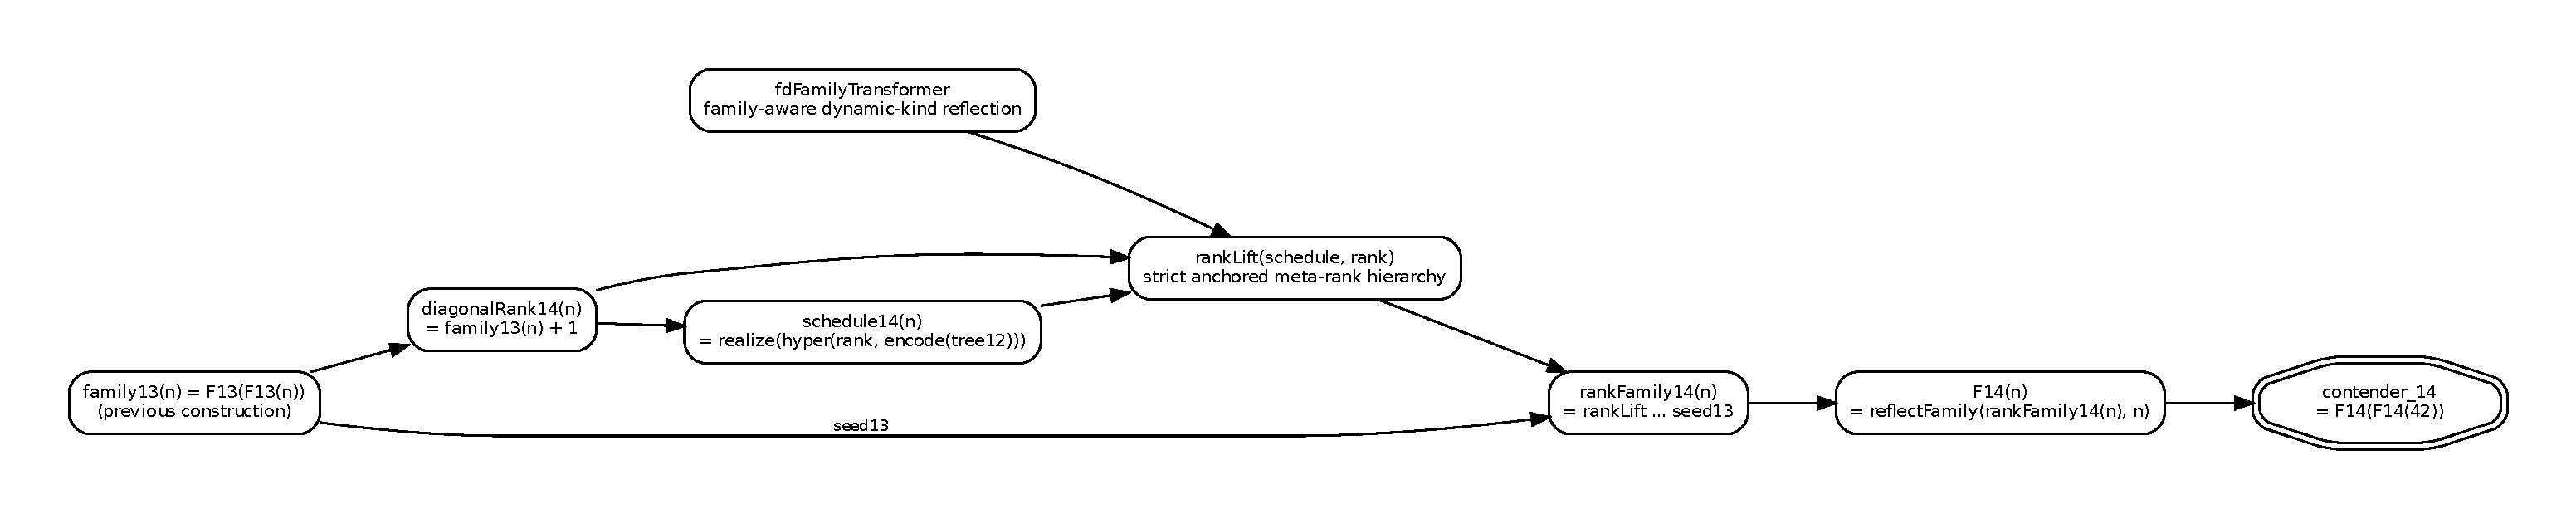
\includegraphics[width=\textwidth]{../artifacts/dependency_graph.pdf}
\caption{Data flow of the proposed Contender~14.  The previous construction
controls the seed, meta-rank, and autonomous schedule; the complete ranked
family is closed by one more family-aware dynamic-kind reflection.}
\label{fig:dependency}
\end{figure}

%======================================================================
\section{Formal comparison with Contender 13}

The central comparison is deliberately short because the generic machinery
carries the complexity.

\begin{lemma}[Seed below ranked family]
For every \(n\),
\[
  \lean{family13}(n)<H_{14}(n)(0,n).
\]
\end{lemma}

\begin{proof}
The transformer \(T_{\mathrm{Fd}}\) is progressive.  Every finite
\(\mathsf{rankLift}\) built from a progressive base is progressive.  Apply that
property to seed coordinate zero, output coordinate zero, and input \(n\):
\[
  s_{13}(0,n)<
  \mathsf{rankLift}_{a_{14}(n)}(r_{14}(n))
    (T_{\mathrm{Fd}})(s_{13})(0,n).
\]
The left side unfolds to \lean{family13 n}; the right side unfolds to
\lean{rankFamily14 n 0 n}.
\end{proof}

\begin{lemma}[Ranked family below the closing reflection]
For every \(n\) and every \(i\le n\),
\[
  H_{14}(n)(i,n)<F_{14}(n).
\]
\end{lemma}

\begin{proof}
This is the visible oracle bound for \(\RFd\), because
\(F_{14}(n)=\RFd(H_{14}(n),n)\).
\end{proof}

\begin{theorem}[Pointwise dominance]
\label{thm:pointwise}
For every \(n\),
\[
  \lean{family13}(n)<F_{14}(n).
\]
\end{theorem}

\begin{proof}
Compose the two preceding strict inequalities at coordinate zero.
\end{proof}

This is stronger than the one-off statement \(C_{13}<C_{14}\): it proves that
the full function underlying Contender~13 is pointwise below the new function.

The input bound for Contender~13 gives
\[
  n<F_{13}(n)<F_{13}(F_{13}(n))=\lean{family13}(n).
\]
Combining this with Theorem~\ref{thm:pointwise} yields
\[
  n<F_{14}(n).
\]
At \(n=42\),
\[
\begin{aligned}
C_{13}
 &=\lean{family13}(42)\\
 &<F_{14}(42)\\
 &<F_{14}(F_{14}(42))\\
 &=C_{14}.
\end{aligned}
\]
Thus the required comparison is obtained.

\begin{theorem}[Proposed Lean comparison]
The supplied source states and proves
\[
  \lean{contender\_13\_lt\_contender\_14}:
  \lean{contender\_13 < contender\_14}.
\]
\end{theorem}

\begin{caution}
The theorem source is complete and contains no placeholder, but this document
does not label it ``kernel checked'' because Lean was unavailable in the
artifact-building sandbox.  The exact command needed for kernel replay is
included in \lean{scripts/check14.py}.
\end{caution}

%======================================================================
\section{Additional formal margins}

The proposal includes more than the minimum comparison theorem.

\subsection{Every successor rank is strictly larger}

Theorem~\ref{thm:rank-step} is formalized as
\lean{rankLift\_step\_lt}.  This is a local theorem at every numerical input,
not an asymptotic heuristic.  It demonstrates that setting the rank to
\(r_{14}(n)\) has genuine order-theoretic meaning.

\subsection{The diagonal rank escapes every fixed finite rank}

The input-growth theorem for \lean{family13} gives, whenever \(k\le n\),
\[
  k\le n<\lean{family13}(n)<\lean{family13}(n)+1=r_{14}(n).
\]
The included Lean theorem is
\lean{fixed\_rank\_lt\_diagonalRank14}.  Consequently no fixed finite
meta-rank captures the diagonal rank function on all sufficiently large
inputs.  This statement concerns the rank index itself.  Combined with strict
successor-rank separation, it explains why the construction is not equivalent
to choosing a large but fixed stack in advance.

\subsection{Final-layer program domination}

For every \(t\in\lean{Fd.ctmsUpTo}(n)\),
\[
\lean{Fd.fvalue}(\lean{packFamily}(H_{14}(n)),n,t)<F_{14}(n).
\]
This is \lean{fvalue\_lt\_F14}.  Substituting \(n=F_{14}(42)\) gives
\lean{fvalue\_lt\_contender\_14}.  It says that the final contender exceeds
every enumerated dynamic-kind program at the final syntax budget, when that
program is allowed to query the entire rank-diagonal family through the packed
oracle.

%======================================================================
\section{Why the increase is significant}

``Significant'' should not be justified by rhetoric about enormous decimal
expansions.  Four structural facts distinguish Contender~14 from Contender~13.

\paragraph{A stronger oracle interface.}
Contender~13 reflects over one unary function \lean{family12}.  The new base
reflection exposes a countable family to dynamic-kind programs.  Programs can
compute the pairing code and query arbitrary family coordinates.  The explicit
prefix maximum simultaneously gives the comparison proof access to all visible
coordinates.

\paragraph{A new type level of amplification.}
Contender~12 operates on transformers.  Contender~14 treats operations on
transformers as first-class mathematical objects, iterates them on W-trees,
and then iterates an anchored promotion by natural rank.  This is not a larger
syntax budget for the same finite maximum; it is a new closure hierarchy.

\paragraph{The rank is previous-number controlled.}
A fixed rank, however elaborate, is still a fixed finite composition.  Here
\(r_{14}(n)=\lean{family13}(n)+1\).  The rank escapes every fixed finite bound,
and each successor rank has a formal strict separation theorem.

\paragraph{The schedule is independently diagonalized.}
The autonomous schedule is also raised through
\(r_{14}(n)\) higher derivatives above \lean{tree12}.  This provides a second
axis of growth rather than using the rank merely to repeat one fixed schedule.
No exact ordinal identity is asserted for this syntax; its role is to supply a
well-founded, computable family of increasingly nested tree schedules.

\paragraph{A final reflective closure.}
The rank-diagonal family is not simply read at one coordinate.  It becomes the
oracle family for another complete dynamic-kind reflection.  Thus the final
result directly dominates visible ranked values and all enumerated programs
relative to that ranked oracle.

These features give both a formal margin and a qualitative one.  The formal
margin is Theorem~\ref{thm:pointwise}.  The qualitative margin is the move from
one dynamic-kind reflection to a previous-number-indexed hierarchy of
strictly separated meta-reflections, followed by another dynamic-kind
reflection.

%======================================================================
\section{Computability and constructiveness}

The number is not practically evaluable, but practical evaluability is not the
contest's criterion.  The correct question is whether the definition denotes a
total recursive natural number without nonconstructive data.

\begin{proposition}[Computability in principle]
Assuming the totality theorems already formalized for the repository's
object-language evaluator, \lean{contender\_14} is a computable natural number.
\end{proposition}

\begin{proof}[Construction audit]
Each component is total for a direct reason.

\begin{enumerate}[leftmargin=*,label=\arabic*.]
\item \lean{Fd.ctmsUpTo n} is generated by primitive recursion and is finite.
\item \lean{Fd.fvalue} invokes the repository's certified normalizer on a term
  accepted by its type checker; otherwise it returns zero.
\item \lean{packFamily} uses primitive recursive arithmetic, including the
  2-adic valuation with a structurally justified decreasing argument.
\item \lean{Fd.reflectFamily} takes maxima over finite lists and a finite
  prefix of the oracle family.
\item \lean{metaStage} is structural recursion on a W-tree.
\item \lean{rankLift} is primitive recursion on a natural number.
\item \lean{Autonomous.hyper} is primitive recursion on the derivative level;
  \lean{Autonomous.realize} is structural recursion on the resulting notation.
\item \lean{F14} composes these total functions, and
  \lean{contender\_14} applies \lean{F14} twice to 42.
\end{enumerate}

No definition requires deciding an arbitrary proposition, choosing an element
of an arbitrary inhabited type, consulting an external oracle, or postulating
termination.  Therefore the closed term computes a natural number in
principle.
\end{proof}

The source-level audit strips comments and strings and checks the definition
modules for the following prohibited tokens:
\begin{center}
\begin{tabular}{lllll}
\lean{noncomputable} & \lean{partial} & \lean{unsafe} & \lean{opaque} & \lean{extern}\\
\lean{implemented\_by} & \lean{sorry} & \lean{admit} & \lean{Classical.choice} & \lean{native\_decide}
\end{tabular}
\end{center}
It also checks that no earlier contender constant occurs in the new definition
modules.  That audit passed.  It is intentionally not represented as a
substitute for kernel checking.

%======================================================================
\section{Axiom and dependency discipline}

The focused audit file performs two kernel-level checks when replayed.

First, it requests \lean{\#print axioms} for the final definition and the
principal theorems.  The build harness accepts only \lean{propext} and
\lean{Quot.sound}, matching the repository policy.

Second, it computes the transitive constant closure of
\lean{BusyLean.contender\_14} and rejects any occurrence of
\lean{contender\_5} through \lean{contender\_13}.  This is stronger than a
text search: it traverses the types and values of every reachable declaration.
The expected closure contains the previous \emph{constructions}---notably
\lean{F13}, \lean{F12}, the normalizers, and the W-tree infrastructure---but
not the previous contender constants.

The distinction matters.  A definition such as
\(\lean{contender\_13}+1\) would pass a numerical comparison but violate the
spirit and explicit rules of the contest.  By contrast,
\(\lean{family13}(n)=F_{13}(F_{13}(n))\) exposes the reusable growth function
at arbitrary input and permits a pointwise theorem.

%======================================================================
\section{Implementation layout}

The overlay adds three library modules.

\begin{description}[leftmargin=3.3cm,style=nextline]
\item[\lean{HyperReflection.lean}]
Defines meta-transformers, tree iteration, anchored rank promotion, finite
rank lifting, progressivity preservation, and strict rank separation.

\item[\lean{Contender14.lean}]
Defines family-aware dynamic-kind reflection, the previous family, diagonal
rank, diagonal schedule, ranked oracle family, \lean{F14}, and
\lean{contender\_14}.

\item[\lean{Comparison14.lean}]
Proves the direct reflection inequalities, progressivity, pointwise dominance,
input growth, the main comparison, rank escape, and program bounds.
\end{description}

The package also adds \lean{test/Audit14.lean} and
\lean{scripts/check14.py}.  The installer appends the three imports to
\lean{BusyLean.lean} without modifying the existing contender files.

The build sequence is intentionally staged:
\[
\lean{BusyLean.Comparison13}
\longrightarrow
\lean{BusyLean.Contender14}
\longrightarrow
\lean{BusyLean.Comparison14}.
\]
The first phase is the accepted baseline.  The second is measured against the
15-second definition budget; the third against the 60-second proof budget.
Both the repository's existing audit and the focused Contender~14 audit then
run under \lean{lake env lean}.

%======================================================================
\section{Validation status and likely proof obligations}

The lack of a Lean executable in the artifact-building environment requires a
clear distinction between source completeness and kernel validation.

\subsection{What was checked}

The source audit verified balanced delimiters after stripping nested comments
and strings; absence of prohibited implementation tokens; absence of earlier
contender constants in the new definition modules; line-length and whitespace
hygiene; and deterministic file hashes.  The mathematical proof structure was
cross-checked against the exact signatures of these audited repository lemmas:
\begin{center}
\begin{tabular}{ll}
\lean{spliceTransformers\_progressive} & \lean{liftTransformer\_progressive}\\
\lean{transformer\_lt\_lift\_at} & \lean{W.le\_prefixMax}\\
\lean{W.le\_maximum} &
\end{tabular}
\end{center}

\subsection{What kernel replay must confirm}

Lean replay must confirm elaboration of the recursive theorem
\lean{metaStage\_progressive}; reduction of the anchored coordinate in
\lean{rankLift\_step\_lt}; definitional equalities connecting
\lean{family13 42} with \lean{contender\_13}; and the expected axiom closure.
These are ordinary elaboration obligations rather than gaps in the mathematical
argument, but they remain real acceptance conditions.

\subsection{Performance risk}

The definitions are deliberately written so that type checking does not
normalize the enormous ranks.  The rank appears as a symbolic argument to
primitive recursion, and proofs use generic induction theorems.  Nevertheless,
Lean's elaborator may unfold more than expected while resolving definitional
equalities, particularly in the strict-rank theorem's final simplification.
The included build harness measures the exact cost.  If optimization is needed,
the first response should be to replace broad simplification with two explicit
\lean{change} steps, not to weaken the construction.

%======================================================================
\section{Informal growth interpretation---and its limits}

It is tempting to assign a named proof-theoretic ordinal to every contender.
That temptation should be resisted here.  The exact strength of the
repository's dynamic-kind language, its interaction with packed external
oracles, and the higher-type autonomous reflection hierarchy has not been
calibrated in a published ordinal analysis.  The present formal result does not
need such a calibration.

A safe qualitative description is available.  Contender~13 takes one bounded
maximum over dynamic-kind programs relative to a previous oracle.  Contender~14
uses the same language as a progressive transformer over a countable family,
builds a strictly increasing hierarchy of operations on that transformer,
selects a rank larger than the previous contender's family value, independently
raises the tree schedule by the same value, and then reflects once more over
the whole result.  Any exact fast-growing-hierarchy assignment would have to
model all of those closures.  The direct Lean inequalities are therefore the
primary mathematics; ordinal terminology is at most a guide for future work.

%======================================================================
\section{Potential refinements after kernel replay}

The current proposal aims for a strong construction with a compact proof
surface.  Several refinements could increase either mathematical clarity or
growth strength.

\subsection{Transitive rank comparison}

The supplied theorem compares rank \(r\) with rank \(r+1\).  An induction can
package this as strict monotonicity in the rank argument at canonical
coordinate zero:
\[
  r<s\Longrightarrow
  \mathsf{rankLift}_a(r)(B)(s_0)(0,n)
  <
  \mathsf{rankLift}_a(s)(B)(s_0)(0,n).
\]
This would combine directly with
\lean{fixed\_rank\_lt\_diagonalRank14} to show that the diagonal ranked family
strictly dominates every fixed rank, pointwise beyond the rank index.

\subsection{Coordinate-sensitive positive branches}

The present positive coordinates of \lean{rankStep} repeat the same scheduled
meta-stage.  One can instead let coordinate \(j+1\) use a schedule transformed
by \(j\), for example an additional autonomous derivative or a selected child
of the schedule.  The preservation proof is unchanged provided every branch
is progressive.  This would make the countable splice carry genuinely distinct
scheduled amplifiers.

\subsection{A hierarchy of dynamic universes}

Contender~13 uses one predicative dynamic kind whose elements range over
closed dyn-free kinds.  A natural language-level extension is a finite tower
\(\mathsf{dyn}_0,\ldots,\mathsf{dyn}_k\), where
\(\mathsf{dyn}_{j+1}\) packages values from kinds containing lower dynamic
levels but not itself.  Diagonalizing over \(k\) would strengthen the object
language rather than only the surrounding amplifier.  Such an extension would
require a new normalization proof and is therefore a larger research project.

\subsection{Internal tree generation}

The current dynamic-kind language has no set-theoretic W-tree value that can be
returned to Lean.  A language combining the dynamic universe with a strictly
positive tree universe could generate its own meta-reflection schedules.  The
main challenge is a predicative semantic model supporting large elimination
without collapsing into an inconsistent type-in-type system.

\subsection{Exact ordinal analysis}

A worthwhile theoretical project is to isolate a transparent subsystem of the
rank-reflection hierarchy and assign an ordinal notation with proved upper and
lower bounds.  The anchor construction may be useful because it exposes a
canonical embedding from each rank into the next.  Any such analysis should be
kept separate from the Lean comparison theorem until the semantic assumptions
are fully explicit.

%======================================================================
\section{Reproduction protocol}

Starting from the audited BusyLean commit, unpack this archive and run:

\begin{lstlisting}[language={},basicstyle=\ttfamily\small]
cd BusyLean_Contender14_RankDiagonal
./install.sh /path/to/BusyLean
cd /path/to/BusyLean
python3 scripts/check14.py
\end{lstlisting}

The installer is idempotent.  It copies the three Lean modules, the focused
audit, and the build script, then appends imports to \lean{BusyLean.lean} only
when they are absent.  The same changes are available as a unified patch for
manual review.

A successful run should establish all of the following:
\begin{enumerate}[leftmargin=*]
\item the accepted baseline through \lean{Comparison13} builds;
\item the new definition module builds within 15 seconds;
\item the comparison module builds within 60 seconds;
\item the repository audit still succeeds;
\item the Contender~14 axiom outputs contain no forbidden axiom;
\item the transitive closure of \lean{contender\_14} contains no earlier
  contender constant.
\end{enumerate}

The actual timing output and axiom report should be committed alongside any
integration pull request.  If the base repository has moved beyond the audited
commit, review the current contender first rather than mechanically applying
the patch.

%======================================================================
\section{Conclusion}

Contender~14 is designed to be a genuine next step in the architecture of
BusyLean.  It does not rely on adding one, increasing a fixed syntax budget, or
reusing the previous constant.  It upgrades the dynamic-kind oracle to a
family, lifts autonomous reflection to meta-transformers, makes every rank
increment formally strict, diagonalizes both rank and schedule by the previous
construction, and closes the result with another dynamic-kind reflection.

The formal comparison has a clean spine:
\[
  \lean{family13}(n)
  < \lean{rankFamily14}(n)(0,n)
  < F_{14}(n),
\]
followed by input growth and the usual outer diagonal.  The strongest claims
are therefore exact inequalities, not informal ordinal labels.  The package is
ready for the one remaining acceptance step: replay under the repository's
pinned Lean~4.34.0 toolchain and measurement against the contest budgets.

%======================================================================
\appendix
\section{Complete Lean source: meta-reflection hierarchy}
\lstinputlisting{../overlay/BusyLean/HyperReflection.lean}

\section{Complete Lean source: Contender 14 definition}
\lstinputlisting{../overlay/BusyLean/Contender14.lean}

\section{Complete Lean source: comparison theorems}
\lstinputlisting{../overlay/BusyLean/Comparison14.lean}

\section{Focused audit source}
\lstinputlisting{../overlay/test/Audit14.lean}

%======================================================================
\begin{thebibliography}{99}

\bibitem{BusyLean}
V.~Reshetnikov and contributors,
\emph{BusyLean: name the biggest number, in Lean},
GitHub repository, audited commit
\texttt{1ee50c7d97bbed57a60709f661453c3e213f4db3}, October 2026.
\url{https://github.com/VladimirReshetnikov/BusyLean}

\bibitem{Roux}
C.~Roux,
\emph{name-the-biggest-number},
GitHub repository.
\url{https://github.com/codyroux/name-the-biggest-number}

\bibitem{Aaronson}
S.~Aaronson,
\emph{Who Can Name the Bigger Number?}
\url{https://www.scottaaronson.com/writings/bignumbers.html}

\bibitem{Girard}
J.-Y.~Girard,
\emph{Interpr\'etation fonctionnelle et \'elimination des coupures de
l'arithm\'etique d'ordre sup\'erieur},
Th\`ese d'\'Etat, Universit\'e Paris VII, 1972.

\bibitem{Reynolds}
J.~C.~Reynolds,
Types, abstraction and parametric polymorphism,
in \emph{Information Processing 83}, pp.~513--523, 1983.

\bibitem{ProofsTypes}
J.-Y.~Girard, Y.~Lafont, and P.~Taylor,
\emph{Proofs and Types},
Cambridge University Press, 1989.

\bibitem{LeanRecursion}
Lean developers,
\emph{The Lean Language Reference: Recursive Definitions and Inductive Types},
Lean~4 documentation.
\url{https://lean-lang.org/doc/reference/latest/Definitions/Recursive-Definitions/}

\bibitem{LeanRelease}
Lean developers,
\emph{Lean 4.34.0 release}, September 14, 2026.
\url{https://github.com/leanprover/lean4/releases/tag/v4.34.0}

\end{thebibliography}

\end{document}
